\vspace{1em}

\usetikzlibrary{graphs, positioning, quotes, shapes.geometric}

\begin{document}
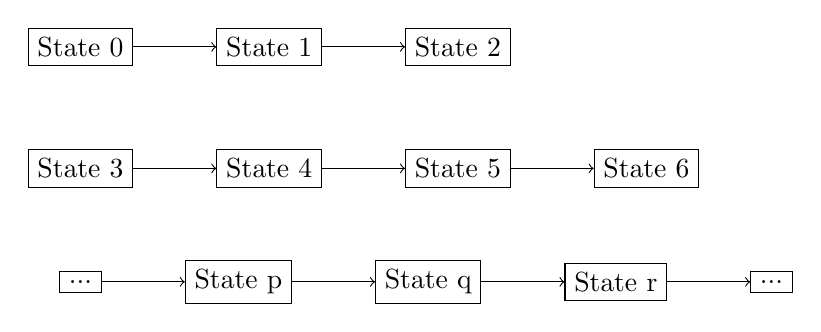
\begin{tikzpicture}[node distance=10pt]
    \node[draw]                           (State 0)  {State 0};
    \node[draw, right=30pt of State 0]    (State 1)  {State 1};
    \node[draw, right=30pt of State 1]    (State 2)  {State 2};
    
    \node[draw, below=30pt of State 0]    (State 3)  {State 3};
    \node[draw, right=30pt of State 3]    (State 4)  {State 4};
    \node[draw, right=30pt of State 4]    (State 5)  {State 5};
    \node[draw, right=30pt of State 5]    (State 6)  {State 6};


    \node[draw, below=30pt of State 3]    (another)  {...};
    \node[draw, right=30pt of another]    (State p)  {State p};
    \node[draw, right=30pt of State p]    (State q)  {State q};
    \node[draw, right=30pt of State q]    (State r)  {State r};
    \node[draw, right=30pt of State r]    (others)  {...};

    \graph{
        (State 0) -> (State 1) -> (State 2);
        (State 3) -> (State 4) -> (State 5) -> (State 6);
        (another) -> (State p) -> (State q) -> (State r) -> (others);
    };
\end{tikzpicture}